\documentclass[red,handout]{beamer}
\usetheme{Dresden}
%\usepackage{caption}
%\DeclareCaptionType{copyrightbox}
\graphicspath{{../figures/}}
% \usepackage{subcaption}
% \captionsetup{compatibility=false}
\usepackage{subfig}
\usepackage{graphicx}
\usepackage{multirow}
\usepackage{amsmath, amsfonts, amssymb}
\usepackage[utf8]{inputenc}
\inputencoding{utf8}
\usepackage{paralist}
\newcommand{\then}{\Rightarrow}
\newcommand{\softor}{\operatornamewithlimits{\tilde{\vee}}}
\newcommand{\softand}{\operatornamewithlimits{\tilde{\wedge}}}
\newcommand{\softthen}{\operatornamewithlimits{\tilde{\then}}}
\newcommand{\softneg}{\operatornamewithlimits{\tilde{\neg}}}


\begin{document}

\title[Planned Protest]{Planned Protest Modeling in News and Social Media}
\subtitle{\tiny Sathappan Muthiah, Bert Huang, Jaime Arredondo, \\
Daved Mares, Lise Getoor, Graham Katz, Naren Ramakrishnan}
\author[S.Muthiah]{Presented by \\
Sathappan Muthiah}
\institute[DAC]
{ 
    \inst{1} Discovery Analytics Center (DAC)\\
    Department of Computer Science\\
    Virginia Tech
}

\titlegraphic{\centering \includegraphics[width=2cm]{vt-logo}
}

\date{January 27, 2015}
%slide 1
\frame{\titlepage}

\section{EMBERS}
%slide 2
\begin{frame}
    \frametitle{Early Model Based Event Recognition Using Surrogates (EMBERS)}
    \begin{itemize}[<+->]
        \item
            Funded by IARPA under the Open Source Indicators (OSI) program
            \begin{itemize}
                \item 
                    To develop automated techniques for continuous analysis of open source data(publicly available)
                    to predict population level events
            \end{itemize}
        \item
            Research and Development project starting April 2012

        \item
            Geographical focus: Latin America

    \end{itemize}
\end{frame}


\section{Problem Overview}
%slide 3
\begin{frame}
    \frametitle{This Paper}
    \begin{itemize}[<+->]
        \item
            Detecting Future time mentions in relevant media to build a protest forecasting system
            \begin{itemize}
                \item
                    Extract `when` and `where` of the protest event
            \end{itemize}
        \item
            Investigate selective superiorities of different social media
            \begin{itemize}[<+->]
                \item
                    News and Blogs (RSS feeds)
                \item
                    Twitter and links extracted from tweets
                \item
                    Facebook
            \end{itemize}
    \end{itemize}
\end{frame}

%slide 4
\begin{frame}
    \frametitle{Motivation}
    \begin{itemize}[<+->]
        \item
            Around 75\% of the protests are planned, organized, or announced in advance
        \item
            Identifying these planned protests is an easy way to forecast protests
    \end{itemize}
\end{frame}

%slide 5
\begin{frame}
    \frametitle{Key Contributions}
    \begin{itemize}[<+->]
        \item
            Real-Time Prospective Study - most studies until now have been retrospective
            \begin{itemize}
                \item
                    Deployed in production since March 2013
            \end{itemize}
        \item
            Semi-Automatic approach for learning keyphrase filters
        \item
            Handling mutliple sources (News, Blogs, Twitter, Facebook)
        \item
            Reasoning about locations
        \item
            Handling relative dates - some recent work use only absolute dates
    \end{itemize}
\end{frame}


\section{Data Sources}
%slide 6
\begin{frame}
\frametitle{Overall Framework}
\begin{figure}
    \centering
    \includegraphics[height=0.6\textheight,width=\textwidth]{pipeline}
\end{figure}
\end{frame}

%slide 7
\begin{frame}
\frametitle{Long Text Sources}
\begin{columns}
\column{0.7\textwidth}
    \begin{itemize}
        \item<1->
            RSS Feeds
            \begin{itemize}
            \item<2->
                Total 9498 different RSS feeds - 6236 news sources and 3262 blogs
            \item<3->
                Duration: November 2012 to present
            \item<4->
                Google/Talkwalker Alerts
            \end{itemize}
        \item<5->
            Twitter-URL
            \begin{itemize}
             \item<6->
                    URL's mentioned are fetched \\
                    and used as a separate source.
            \end{itemize}
    \end{itemize}
    \column{0.3\textwidth}
    \begin{inparaenum}
        \only<2->{\item \includegraphics[width=0.3\textwidth,height=0.2\textheight]{rss}}
            \vspace{.5em}
        \only<4->{\item \includegraphics[width=0.3\textwidth]{alerts}}
            \vspace{.5em}
        \only<5->{\item \includegraphics[width=0.4\textwidth]{twitter-url}}
    \end{inparaenum}
\end{columns}
\end{frame}

%slide 8
\begin{frame}
\frametitle{Short Text Sources}
\begin{columns}
    \column{0.6\textwidth}
    \begin{itemize}
    \item<1->
        Twitter
        \begin{itemize}
            \item<2->
                Duration: November 2012 to present
        \end{itemize}
    \item<3->
        Facebook-Event
        \begin{itemize}
            \item<4->
                Duration: July 2013 to present
        \end{itemize}
    \end{itemize}
    \column{0.3\textwidth}
    \begin{inparaenum}
        \only<1->{\item \includegraphics[width=0.6\textwidth]{twitter}}
        \vspace{2em}
        \only<3->{\item \includegraphics[width=0.6\textwidth]{facebook}}
        \vspace{2em}
    \end{inparaenum}
\end{columns}
\end{frame}

%slide 9
\begin{frame}
    \frametitle{Distribution of Alerts}
    \begin{figure}
        \centering
        \includegraphics[width=0.7\textwidth]{warnings_sources}
    \end{figure}
\end{frame}

%slide 10
\section{Preliminaries}
\begin{frame}
\frametitle{Preliminaries-Probabilistic Soft Logic}
    \begin{itemize}[<+->]
        \item
            Framework for collective probabilistic reasoning in relational domains
        \item
            Uses first order logic rules as a template language for graphical models
        \item
            Soft truth values
        \item
            Applications in collective classification, ontology alignment,opinion diffusion, graph summarization etc
        \item
            A simple PSL rule:
            \begin{figure}
                \includegraphics[scale=0.3]{psl_rule_example}
            \end{figure}
    \end{itemize}
\end{frame}

%slide 11
\section{Linguistic Preprocessing}
\begin{frame}
\begin{columns}
    \frametitle{Linguistic Preprocessing}
    \column{0.5\textwidth}
    \begin{itemize}
        \item<1->
            Natural Language Enrichment
        \begin{itemize}[<+->]
            \item
                Tokenization
            \item
                Lemmatization
            \item
                Noun Phrase Extraction
            \item
                Named Entity Extraction and Classification
        \end{itemize}
        \item<6->
            TIMEN Enrichment
        \begin{itemize}
            \item
                Extraction of Absolute Dates from text
            \item
                Identification of Relative dates like `yesterday, next wednesday' etc
        \end{itemize}
    \end{itemize}

    \column{0.3\textwidth}
    \only<1-5>{\includegraphics[scale=0.25]{basis_enrichment}}
    \only<6>{\includegraphics[scale=0.3]{timen_enrichment}}
\end{columns}
\end{frame}

\section{Geocoding}
%slide 12
\begin{frame}
    \frametitle{Geocoding - RSS Feeds (contd...)}
    \begin{itemize}[<+->]
        \item Primary rules
        \begin{flalign*}
            ENTITY&(L, location) \softand REFERSTO(L, locID) &\\
                                &\rightarrow PSLLOCATION(Article, locID) &
        \end{flalign*}


        \begin{flalign*}
            ENTITY&(C, location) \softand IsCountry(C) &\\
                                &\rightarrow ArticleCountry(Article, C) &
        \end{flalign*}


        \begin{flalign*}
            ENTITY&(S, location) \softand IsState(S)&\\
                                    &\rightarrow ArticleState(Article, S)&
        \end{flalign*}

    \end{itemize}
\end{frame}

%slide 13
\begin{frame}
    \frametitle{Geocoding - RSS Feeds (contd...)}
    \begin{itemize}[<+->]
        \item Secondary rules
    \begin{flalign*}
        ENTITY&(O, organization) \softand REFERSTO(O, locID)&\\
                                &\rightarrow PSLLOCATION(Article, locID) &
    \end{flalign*}


    \begin{flalign*}
        ENTITY&(O, organization) \softand IsCountry(O)&\\
            &\rightarrow ArticleCountry(Article, O)&
    \end{flalign*}


    \begin{flalign*}
        ENTITY&(O, organization) \softand IsState(O)&\\
              &\rightarrow ArticleState(Article, O) &
    \end{flalign*}

    \end{itemize}
\end{frame}

%slide 14
\begin{frame}
\frametitle{Geocoding - RSS Feeds}
\begin{figure}
    \centering
    \includegraphics[width=\textwidth]{psl_pipeline2}
\end{figure}
\end{frame}


%slide 15
\begin{frame}
\frametitle{Geocoding - Twitter and Facebook}
    \begin{itemize}[<+->]
        \item
            Geotag of the tweet or Venue tag in Facebook Events
        \item
            Twitter ``places" metadata
        \item
            Other text fields (user profile, tweet text, Facebook Event Text)
    \end{itemize}
\end{frame}

%slide 16
\section{Phrase Filtering}
\begin{frame}
\frametitle{Phrase List Development}
    \begin{itemize}[<+->]
        \item
            Semi-Automatic
        \item
            Different Lists are built for different Sources
        \item
            Seed phrases are identified from analysis of known planned events from print media.
    \end{itemize}

\end{frame}

%slide 17
\begin{frame}
    \frametitle{Dependency Parsing}
    \begin{figure}
        \includegraphics[width=\textwidth]{phraseLearning}
    \end{figure}
\end{frame}

%slide 18
\begin{frame}
    \frametitle{Phrase List for Long Text}
    \begin{figure}
        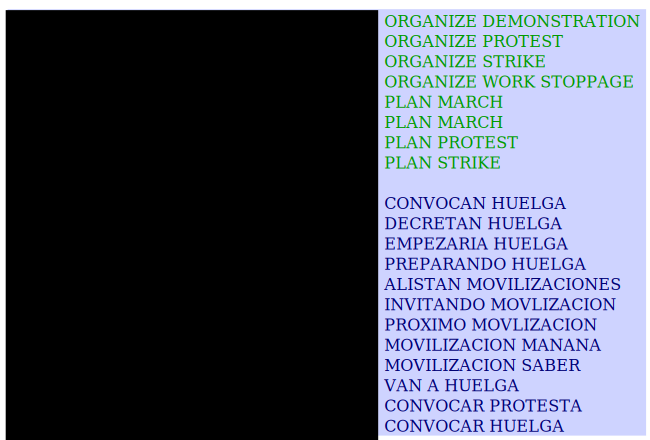
\includegraphics[scale=0.5]{wordlist_rss}
    \end{figure}
\end{frame}


%slide 19
\begin{frame}
    \frametitle{Phrase List for Short text}
     \begin{figure}
        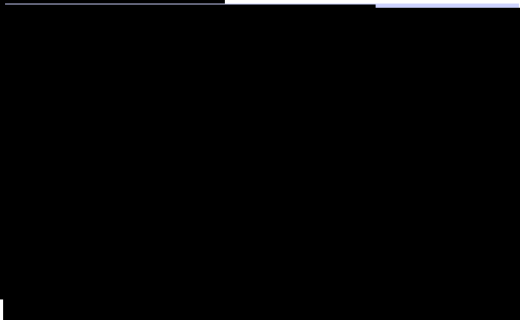
\includegraphics[scale=0.5]{wordlist_twitter}
     \end{figure}
\end{frame}


%slide 20
\begin{frame}
    \frametitle{Phrase Matching}
    \begin{itemize}[<+->]
        \item
            Sample phrase matching rule:
            \begin{figure}
                \includegraphics[scale=0.5]{phrase_rule}
            \end{figure}
        \item
            Linguistically sophisticated and flexible matching
        \item
            Near regex style matching
        \item
            Example matched sentence:
            {\em ``The students are planning a couple of big protests tomorrow"}
    \end{itemize}
\end{frame}


%slide 21
\begin{frame}
    \frametitle{System Framework Once again}
    \begin{figure}
        \centering
        \includegraphics[height=0.6\textheight,width=\textwidth]{pipeline}
    \end{figure}
\end{frame}

\section{Evaluation}

%slide 22
\begin{frame}
\frametitle{Evaluation Methodology}
    \begin{itemize}
        \item
            Bipartite Matching
    \end{itemize}
    \begin{figure}
        \includegraphics[height=0.7\textheight]{matching}
    \end{figure}

\end{frame}

%slide 23
\begin{frame}
    \frametitle{Evaluation Methodology (contd ...)}
    \begin{itemize}
        \item<2->
            Location Score
            \begin{equation*}
                \operatorname{LS}=1 - \frac{\min(\textrm{distance offset}, 300)}{300}
            \end{equation*}
        \item<3->
            Date Score
            \begin{equation*}
                \operatorname{DS}=1 - \frac{\min(\textrm{date offset}, \operatorname{INTERVAL})}{\operatorname{INTERVAL}}
            \end{equation*}

        \item<1->
            Total Quality Score
            \begin{equation*}
                \operatorname{QS}=(\operatorname{DS} + \operatorname{LS})*2
            \end{equation*}
    \end{itemize}
\end{frame}

%slide 24
\begin{frame}
    \frametitle{Warnings vs GSR}
    \begin{figure}%
    \centering
    \subfloat{\includegraphics[width=0.45\textwidth]{gsr_distribution}}%
    \qquad
    \subfloat{\includegraphics[width=0.45\textwidth]{pp_dist}}%
    \end{figure}
\end{frame}

%slide 25
\begin{frame}
     \frametitle{Venezuelan Spring}
     \begin{figure}
        \centering
        \includegraphics[scale=0.4]{venezuela}
     \end{figure}
\end{frame}

%slide 26
\begin{frame}
    \frametitle{Brazilian Spring}
    \begin{figure}
        \centering
        \includegraphics[scale=0.4]{brazil_june}
    \end{figure}
\end{frame}

%slide 27
\begin{frame}
    \frametitle{Individual Source Level Perfomance}
    \resizebox{\linewidth}{!}{
    \begin{tabular}{|*{17}{c|}}
        \hline
        & \multicolumn{4}{ |c| }{News/Blogs} & \multicolumn{4}{ |c| }{Twitter} & \multicolumn{4}{ |c| }{Facebook} & \multicolumn{4}{ |c| }{Combined}\\
        \hline
         & QS & Pr. & Rec. &LT & QS & Pr. & Rec. & LT & QS & Pr. & Rec. & LT & QS & Pr. & Rec. & LT\\
        \hline
        AR &3.14&0.32&0.69&3.94&3.52&{\bf0.78}&0.14&3.14&{\bf3.70}&0.50&0.04&3.00&3.02&0.36&{\bf0.80}&{\bf4.50}\\
        BR &3.14&0.48&0.54&{\bf5.85}&-&-&-&-&{\bf3.62}&{\bf0.76}&0.18&2.46&3.28&0.49&{\bf0.65}&5.15\\
        CL &3.06&0.91&0.67&5.40&{\bf3.52}&{\bf1.00}&0.23&4.29&-&-&-&-&3.16&0.83&{\bf0.80}&{\bf5.92}\\
        CO &2.74&0.90&0.56&{\bf7.44}&3.30&{\bf1.00}&0.15&2.43&{\bf4.00}&{\bf1.00}&0.02&2.00&2.88&0.84&{\bf0.65}&6.47\\
        EC &-&-&-&-&{\bf2.32}&{\bf1.00}&{\bf0.06}&{\bf17.00}&-&-&-&-&{\bf2.32}&{\bf0.50}&{\bf0.06}&{\bf17.00}\\
        MX &2.96&0.88&0.25&{\bf3.69}&3.14&{\bf1.00}&0.02&1.43&{\bf3.72}&0.67&0.01&2.00&3.00&0.87&{\bf0.27}&3.51\\
        SV &{\bf3.22}&{\bf1.00}&{\bf0.03}&{\bf1.0}&-&-&-&-&-&-&-&-&{\bf3.22}&{\bf1.0}&{\bf0.03}&{\bf1.0}\\
        PY &3.38&{\bf1.00}&{\bf0.16}&9.11&3.84&{\bf1.00}&0.04&{\bf11.40}&3.96&{\bf1.00}&0.01&2.00&3.60&0.96&{\bf0.20}&9.35\\
        UY &{\bf3.24}&{\bf1.00}&{\bf0.29}&{\bf2.40}&-&-&-&-&-&-&-&-&3.24&{\bf1.00}&{\bf0.29}&3.24\\
        VE &{\bf3.80}&{\bf1.00}&0.36&{\bf3.27}&3.68&0.97&0.33&2.39&-&-&-&-&3.64&0.99&{\bf0.69}&2.88\\
        ALL &3.34&0.69&0.35&{\bf4.57}&3.62&{\bf0.97}&0.15&2.82&3.66&0.74&0.03&2.44&3.36&0.73&{\bf0.51}&4.08\\
        \hline
    \end{tabular}}
\end{frame}

%slide 28
\begin{frame}
    \frametitle{Performance over time}
    \begin{figure}
        \includegraphics[scale=0.4]{monthlyqs}
    \end{figure}
\end{frame}

%slide 29
\begin{frame}
    \frametitle{Lead-Time vs Quality}
    \begin{figure}
        \includegraphics[scale=0.4]{leadTimeVsQS}
    \end{figure}
\end{frame}

%slide 30
\begin{frame}
    \frametitle{Conclusion and Future Work}
    \begin{itemize}[<+->]
        \item
            Current system capable of detecting planned protests and resolve $(i)$ date and $(ii)$location of an event satisfactorily
        \item
            Different sources have different advantages and superiorities
        \item
            Future work is aimed at three aspects
            \begin{itemize}[<+->]
                \item
                    Address situations involving nationwide protests and systems of protests
                \item
                    Generalize system to be able to make predictions from groups of articles and possibly from different sources
                \item
                    Generalize system to detect not-so-explicitly stated expressions of discontent
                \end{itemize}
        \end{itemize}
\end{frame}

%slide 31
\begin{frame}
    \frametitle{End}
    \center{Thank You!}
\end{frame}


%backup 1
\begin{frame}[noframenumbering]
    \frametitle{Quality Score vs Matching window size}
    \begin{figure}
        \includegraphics[scale=0.4]{matchingwindow}
    \end{figure}
\end{frame}

%backup 2
\begin{frame}[noframenumbering]
    \frametitle{Quality Score Distribution}
    \centering
    \begin{figure}
        \includegraphics[scale=0.6]{doubleHump}
    \end{figure}
\end{frame}

%backup 3
\begin{frame}[noframenumbering]
    \frametitle{Venezuelan Violent Protests}
     \begin{figure}
        \centering
        \includegraphics[scale=0.4]{venezuela_violent}
     \end{figure}
\end{frame}


%backup 4
\begin{frame}[noframenumbering]
    \frametitle{Appendix A}
    \begin{itemize}
        \item  Lukasiewicz t-norm
    \begin{figure}
        \includegraphics[scale=0.4]{luke_norm}
    \end{figure}
    \item Distance to Satisfaction
    \begin{figure}
        \includegraphics[scale=0.4]{dis_sat_psl}
    \end{figure}
\end{itemize}

%backup 5
\end{frame}
\begin{frame}[noframenumbering]
    \frametitle{PSL MPE Inference}
    \begin{itemize}
        \item Lukasiewicz t-norm is used to determine the degree to which a ground rule is satisfied
        \item Most Probable Explanation or Inference (MPE): Inferring the most likely values for a proposition given values of remaining propositions
            \begin{figure}
                \includegraphics[scale=0.4]{psl_equation}
            \end{figure}
        \item Here,
            $I$ is an interpretation of the proposition,

            $\lambda_r$ is the weight of the rule,

            $d_r(I)$ is the distance to satisfaction of the rule (degree to which the condition/rule is violated)
        \end{itemize}
\end{frame}

\end{document}
